\section{Experiments and Evaluation}
\label{sec:exp}
In this section, we present our experimental methodology, evaluation metrics and the results of the experiments.

\subsection{Sentiment Analysis}
\label{sec:sent-exp}
In order to measure the performance of different classification techniques on the YouTube data, we split the data from US comments into train and test subsets. To generate the train set, we randomly choose $80\%$ of the comments from each of the three categories. The remaining comments form the test set. We use $20\%$ of the GB comments as development set. 
Table~\ref{tab:accuracy} shows the accuracy measured on train and test sets. Naive Bayes classifier has the worst performance among all methods. This result is predictable as the conditional independence condition required by the Naive Bayes classifier is not satisfied in this dataset. In particular, the probability of two words happening in a comment given the category of the comment are not independent from one another. On this dataset, SVM classifier has the best performance.

\begin{table}%
\centering
\begin{tabular}{|l|c|c|}
\hline
Model & Dev Accuracy & Test Accuracy \\
\hline
Logistic Regression & $0.709$ & $0.709$ \\
\hline
Bernoulli NB & $0.709$ & $0.715$ \\
\hline
Ridge Classifier & $0.914$ & $0.905$ \\
\hline
Linear SVC & $0.956$ & $0.951$ \\
\hline
\end{tabular}
\caption{Sentiment classification accuracy of YouTube comments}
\label{tab:accuracy}
\end{table}

Figure~\ref{fig:calibration} shows the calibration curve of the aforementioned techniques. It is observed that Naive Bayes classifier is not well-calibrated over the range $[0,1]$. From among the remaining three methods, Logistic Regression is well-calibrated over the range $[0,1]$ and is in general better calibrated than the other two methods.
\begin{figure}[h]
\centering
\begin{minipage}{0.49\textwidth}
\centering
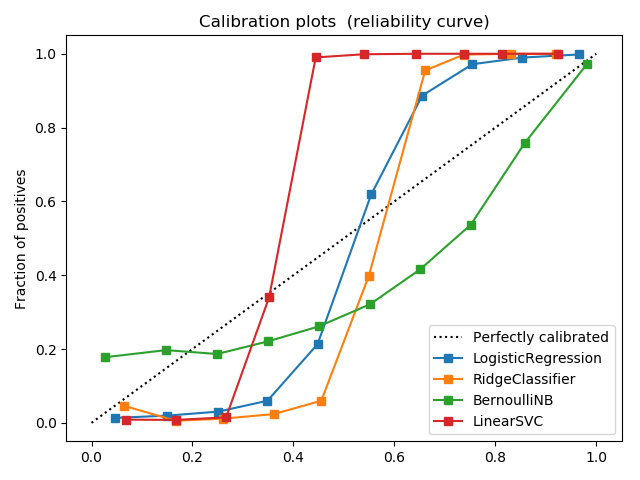
\includegraphics[width=1.0\linewidth]{figures/calibration.png}
\caption{Word cloud for positive comments}
\label{fig:calibration}
\end{minipage}
\begin{minipage}{0.49\textwidth}
\centering
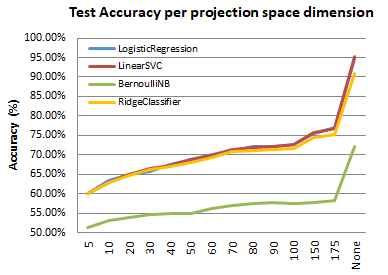
\includegraphics[width=1.0\linewidth]{figures/dim_reduction_accuracy.png}
\caption{Accuracy vs. project space dimensions}
\label{fig:dim-reduction}
\end{minipage}
\end{figure}
\subsection{Effect of Dimensionality Reduction}
\label{sec:dim-reduction}
In this set of experiments, we examined how dimensionality reduction can affect the accuracy of predictions. Dimension reduction is usually applied to reduce the complexity of computations. We apply TruncatedSVD to project TF-IDF features to fewer dimensions than those of the original TF-IDF feature space. We use TruncatedSVD rather than Principal Component Analysis (PCS) because the TF-IDF features are stored in a sparse matrix by the SKLearn library which PCA cannot process. TruncatedSVD is very similar to PCA. However, the data is not centered around its mean in the former.
Figure~\ref{fig:truncatedsvd} shows the accuracy of sentiment analysis with TruncatedSVD applied to TF-IDF features versus number of dimensions of the projection space. It is observed that accuracy increases with the number of dimensions. Nevertheless, with $175$ dimensions, it is still far from the case where no dimensionality reduction is applied. It seems that in this dataset, $175$ dimensions is not enough to project the data without loosing much information. We could not experiment with higher dimensions due to memory limitations of our desktops.

\subsection{Category Classification}
\label{sec:cat-exp}

First, we report the results of experiments for category classification using TF-IDF comment features. In this method we try to detect the category of the video a comment is talking about using the TF-IDF features of the comments. Table~\ref{tab:comment-cat} shows the accuracy of different techniques. It is seen that the results are not as good as sentiment classification. Considering there are $15$ categories versus $3$ sentiment classes, this problem is deemed to be harder. Yet, the probability of a successful random category guess is only $1/15 (6.7\%)$. Consequently, category prediction based on TF-IDF features of comments is still a big improvement over random guessing.
We then conducted category classification based on video tags. Table~\ref{tab:tag-comment} shows accuracy of category classification using tags. It is observed that tags can predict the category with much higher accuracy. Note that tags are considered a property of videos while TF-IDF features are a property of comments. In addition, tags are explicitly chosen to classify the videos. As a result, it is expected that are more directly relevant to the content of the video and are less noisy which lead to better accuracy in category prediction.
 
In another experiment, we examined the effect of the number of categories on the accuracy. Intuitively, the larger the number of categories, the more difficult the classification problem is expected to be. To experiment this intuition, we created a list of categories with ascending order of each category population. We considered the first $2$ categories, that is, the two categories with greatest number of videos, ignored the remaining videos in train and test set and measured the accuracy. The same experiment was repeated for $3, 4, \ldots, 15$ categories.
Figure~\ref{fig:cat-num-test} shows how test accuracy decreases by increasing the number of categories.